\section{Security Protocols} % Message deduction?
Security protocols is an abstract or concrete protocol, that characterise the security related functions and applies cryptographic methods. It describes how the algorithm should be used to ensure the security and integrity of data transmitted. The security protocol is a protocol that runs in an untrusted environment where it assumes channels are untrusted and participants are dishonest. In academic examples, they are often described with the Alice and Bob notation, which will also be used in the following examples to create a better understanding of how security protocols work and can be reasoned about. 

%A way of reason about wether a message is deductible by an adversary is through inference rules. Inference rules offers a formal analysis for proving security properties of protocols. \\ \\
%TODO: discuss how Inference rules and derivation sequences can be used 

\subsection{Needham-Schroeder Protocol}
The Needham-Schroeder Public Key Protocol, was first proposed by Roger Needham and Michael Schroeder in 1978, and will be used as a running example in this and the following two sections. %and is one of the two key transport protocols intended for an insecure network. 

The Needham-Schroeder Public Key Protocol can be illustrated by the before mentioned Alice and Bob notation in the following way, as done by \citeauthor{DBLP:journals/ftpl/CortierK14}

\begin{center}
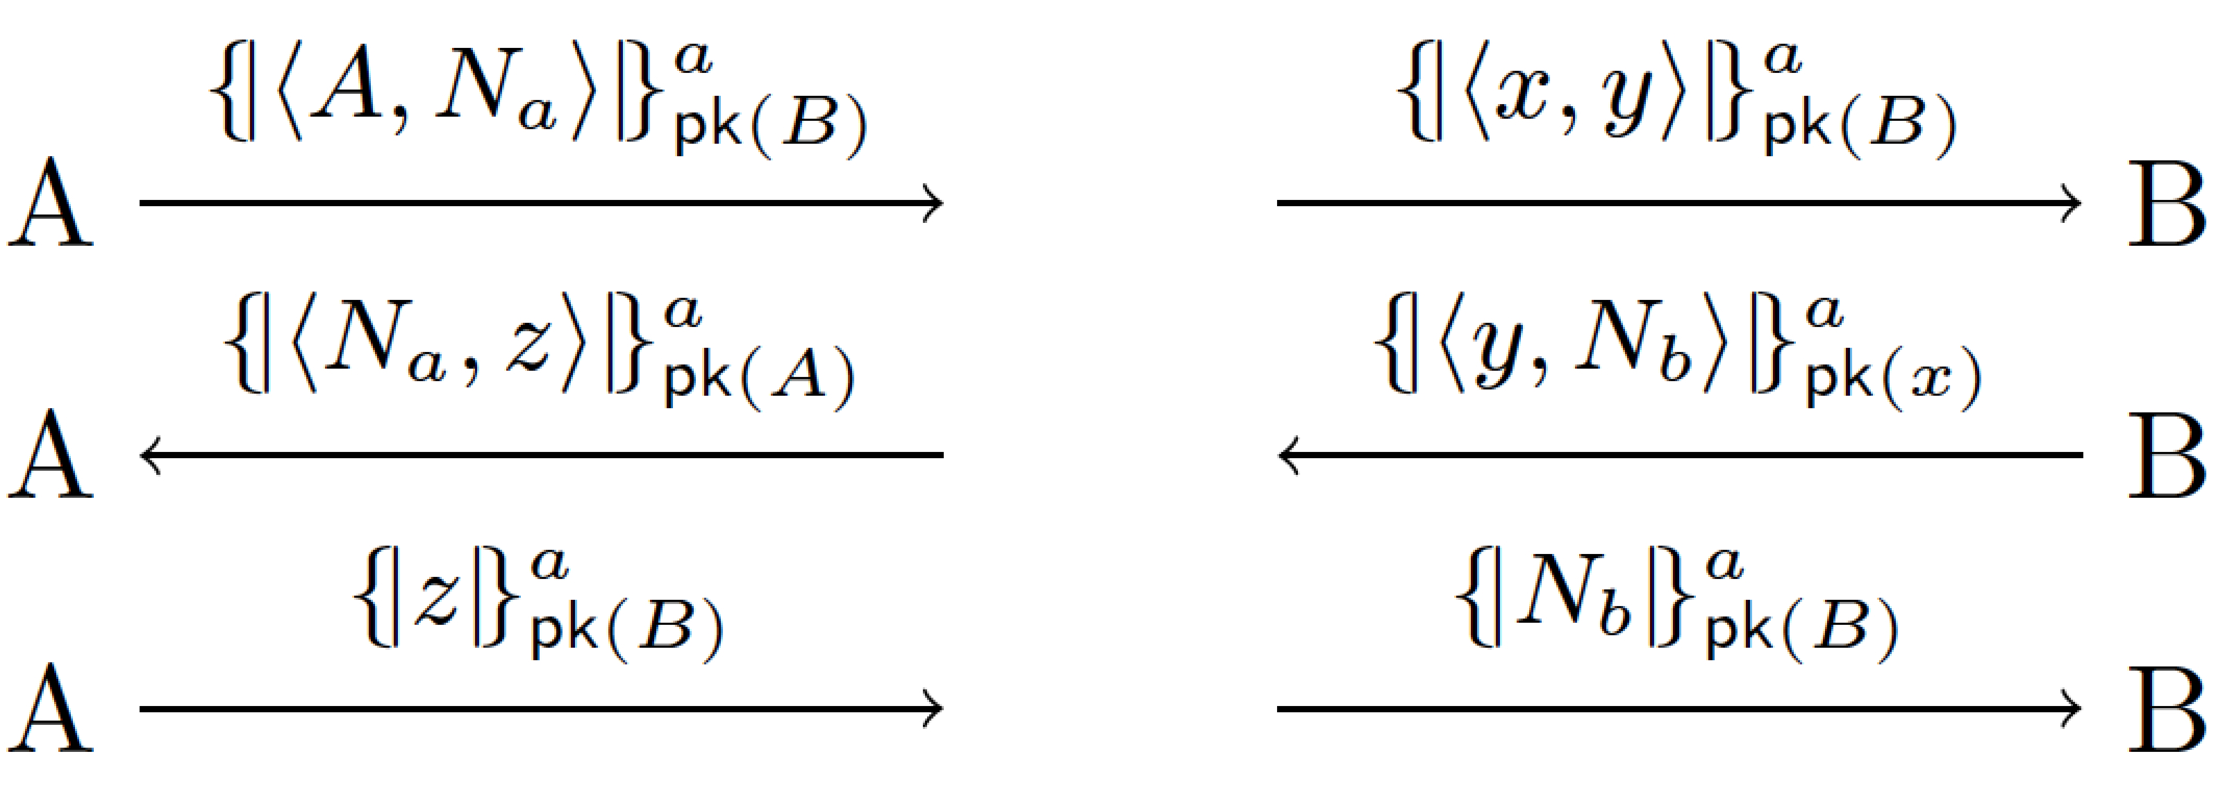
\includegraphics[width=0.6\textwidth, angle=0]{Graphics/NS_Protocol.pdf}
\end{center}

The A and B each represent Alice and Bob, while the arrows indicates the direction of the sent and received messages, by which are illustrated above each line. The notation $\{| m |\}^a_{pk(B)}$ denotes that the message \textit{m} is created with an asymmetric encryption of Bob's public key, while the $\langle m_1, m_2 \rangle$ illustrates a pairing or concatenation of the two messages. The \textit{A} and \textit{B} in the messages each represent the identities of Alice and Bob, while \textit{N$_a$} denotes the freshly generated nonce, a random number generated each session. The variables \textit{x, y, z} are used for the unknown values of the message.

In the first exchange, Alice sends her identity and nonce asymmetrically encrypted with Bob's public key. Bob receives the message, with variables \textit{x} and \textit{y}, illustrating the unknown values of the message. Bob decrypts the message to check that it is well-formed. He then generate his own nonce, pair it with Alice's nonce, and then encrypts it with Alice's public key. Alice then decrypts Bob's message, to verify that it contains her previously sent nonce, which proves that Bob received her first message. 
This way of sending and receiving nonces is often called a \textit{challenge-response} authentication \autocite{DBLP:journals/ftpl/CortierK14}, and is also what you see when using passwords, where the challenger asks for a password and then checks that the response is valid. 
\bigbreak
The gap left between the two participants illustrate the challenge of this protocol in an untrusted network, as an attacker may instigate a \textit{man-in-the-middle} attack. This vulnerability of the protocol, was first described by Gavin Lowe in his paper published in 1995, where also a fix was purposed. Again the Alice and Bob notation is used, but now we introduce an adversary \textit{C}, as illustrated here by \citeauthor{DBLP:journals/ftpl/CortierK14}.

\begin{center}
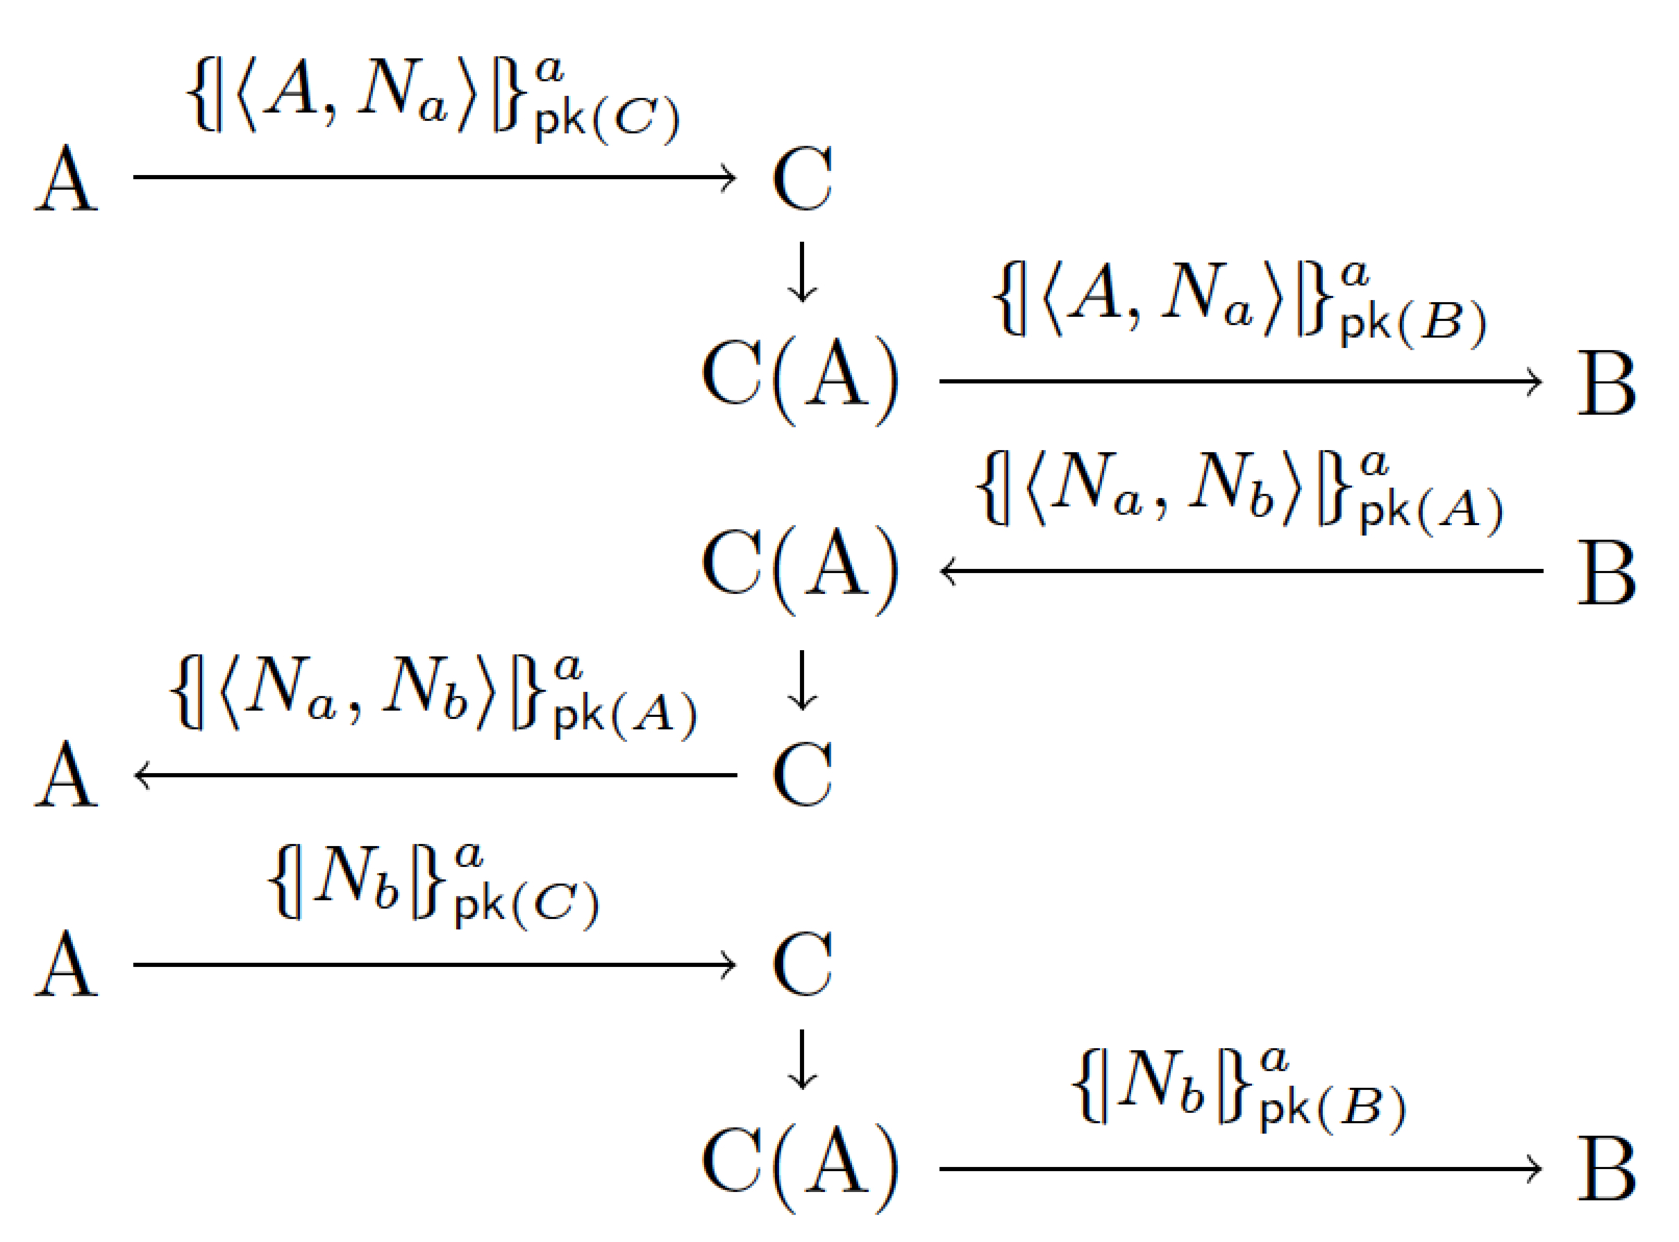
\includegraphics[width=0.55\textwidth, angle=0]{Graphics/Challenge.pdf}
\end{center}

If the attacker can persuade \textit{A} to initiate a session with him, he relay the messages to \textit{B}, and thus convince him he is communicating with \textit{A}. Lowe suggest a simple solution to this problem, by adding the identity of the sender in the second message so that $\{|\langle N_a, N_b\rangle |\}^a_{pk(a)}$ would now look as such $\{|\langle N_a, \langle N_b, B\rangle \rangle |\}^a_{pk(a)}$. To highlight this vulnerability more clearly, I will revisit the Needham-Schroeder protocol again in the Applied Pi-Calculus section, where a more detailed description of why this attack is possible will be shown. 


\iffalse
A -> B : m  			= Alice sends Bob a message
Notation {|m|}^a_pk(B) 	= asymmetric encryption of m with Bob's public key. 
<m1, m2>				= pairing, i.e. concatenation of the two messages
A, B					= Their identities
N_a					= nonce (number used once - fresh random generated each session)
x, y, z				= Variables for unknown component(values)

First 					= Alice sends her identity and nonce, encrypted with Bob's public key

Bob then decrypts and check that it is well-formed.
This mechanism of sending someone an encrypted nonce and waiting for the recipient to send back this nonce is often called a challenge-response mechanism.
Alice then decrypts Bob's message, and verifies that it contains har previous N_a - proves that Bob received first message

The aim of the protocol is to guarantee mutual 'authentication' - ensures they have been communicating with the right person
Moreover, the protocol should guarantee 'confidentiality' of the nonces Na and Nb.
 - Honest execution (man in the middle attack)
\fi

\subsection{Message deduction}
Message deduction is a formal way of figuring out wether a message can be deducted from a priori given set of messages by using induction rules and derivation sequences. Most important is the use of \textit{terms} representing messages. This allows for a better illustration of the keys, identities and nonces, but abstract away the exact values, while still keeping the structure as a special labelled graph. \\ \\
\textbf{Terms} \qquad
Functions symbols such as \textit{f}, are used to capture cryptographic primitives i.e. encryption and one-way hash functions, each assigned with an associated integer as its arity. Function symbols with arity 0 are seen as a constant, while a finite set of functions symbols is called a \textit{signature}. Terms are build by applying function symbols to a infinite set of names \textit{N} (used for keys, nonces or identities), variables \textit{X} and other terms \textit{F}, and can be defined as such \textit{T(F, X, N)}. As can be seen later, variables are often used to represent unknown variables, e.g. components received from another participant of the protocol. \\

\noindent \textbf{Inference rules}  \qquad
%TODO: Introduce the Dolev-Yao model from 1981 - first symbolic formalisation of the deductive power of an attacker
Inference rules uses the following notation $\infer{u} {u_l & ... & u_n}$ with $u_l,...,u_n, u$ as terms with variables. Having a set of inference rules is also called an inference system, and often contains both \textit{composition rules} and \textit{decomposition rules}. Below can be seen an inference system for the Dolev-Yao model ($\mathcal{I}_{DY}$) with the composition rules presented first in each line, and the following decomposition rules. 
\begin{center}
$\mathcal{I}_{DY}\ :$
\begin{math}
  \left\{
    \begin{array}{l l l}
      \infer{\langle x, y \rangle}{x,y} \qquad \infer{x}{\langle x, y \rangle} \qquad \infer{y}{\langle x, y \rangle} \\ \\
      \infer{\text{senc}(x, y)}{x\ y} \qquad  \infer{x}{\text{senc}(x, y)\ y} \\ \\
      \infer{\text{aenc}(x, y)}{x\ y} \qquad \infer{x}{\text{aenc}(x, \text{pk}(y))\ y}
    \end{array}
  \right.
\end{math}
\end{center}
\bigbreak
\noindent In the first line we have the rules for concatenation. It shows that anyone have the possibility of concatenating two terms (first rule), while the next two rules show that it is possible to retrieve the individual terms from a concatenation. 
On the second line we have the rules for symmetric encrypting and decrypting, showing that anyone can decrypt a message if they have the corresponding key. The same goes for the asymmetric encryption and decryption, with the rules shown in the third line. \\

\noindent \textbf{Derivation sequence}  \qquad
By combining inference rule, we are able to derive new messages. An example is given by \citeauthor{DBLP:journals/ftpl/CortierK14} with the set of messages $S = \{\langle k_1, k_2\rangle ,\langle k_3, a\rangle , \{|n|\}^a_{\langle k_1, k_3\rangle}\}$, illustrating how the set can be derived by an attacker through the use of the before mentioned inference rules (here represented by a proof tree):
\begin{center}
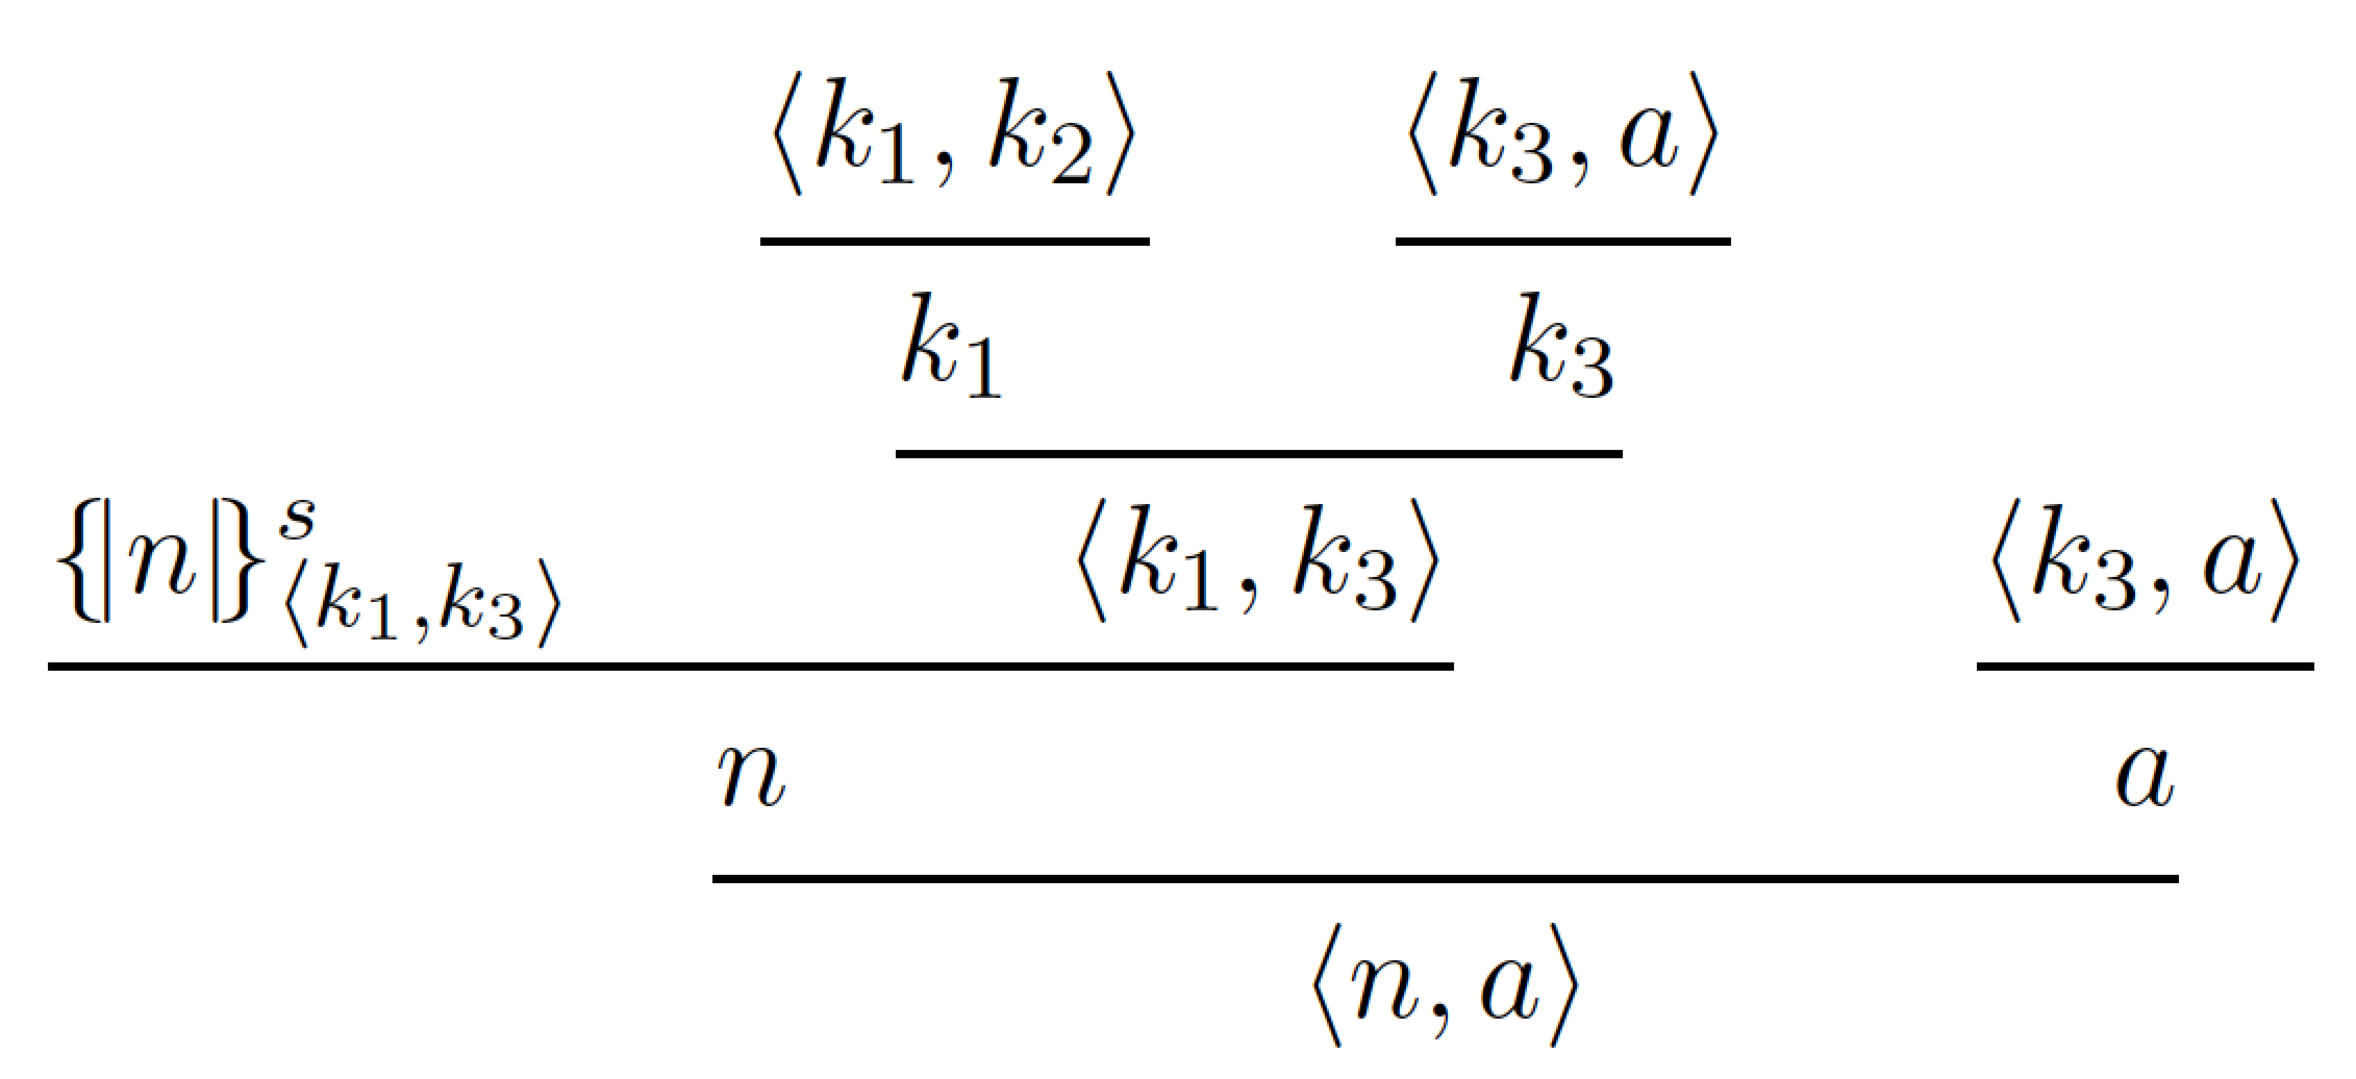
\includegraphics[width=0.55\textwidth, angle=0]{Graphics/Proof_tree.pdf}
\end{center}
From $\langle k1, k2\rangle$ the attacker can use the second rule shown, to learn \textit{k1}. Using the same rule, he is also able to obtain \textit{k3} from $\langle k3, a\rangle$. From these two he is now able to decrypt message \textit{n} from $\{|n|\}^s_{\langle k1, k3\rangle}$, and thus get the encrypted message sent. For further illustration it is shown that the attacker is also able to get hold of \textit{a}, which in turn is called that $\langle n, a\rangle$ is \textit{deducible} from the set of messages $S$. \\ \\


%\subsection{Examples}
%TODO: show examples of a man in the middle attack on the NS and DH protocols: \\ \\
%- Needham-Schroeder Public key protocol (now modified according to Lowe's man in the middle attack): 


